\documentclass[times,t]{beamer}
\usepackage{amssymb}
\usepackage{amsmath}
\usepackage{amsfonts}
\usepackage{lmodern} 
% Calligraphic fonts
\newcommand{\calA}{{\cal A}}
\newcommand{\calB}{{\cal B}}
\newcommand{\calC}{{\cal C}}
\newcommand{\calD}{{\cal D}}
\newcommand{\calE}{{\cal E}}
\newcommand{\calF}{{\cal F}}
\newcommand{\calG}{{\cal G}}
\newcommand{\calH}{{\cal H}}
\newcommand{\calI}{{\cal I}}
\newcommand{\calJ}{{\cal J}}
\newcommand{\calK}{{\cal K}}
\newcommand{\calL}{{\cal L}}
\newcommand{\calM}{{\cal M}}
\newcommand{\calN}{{\cal N}}
\newcommand{\calO}{{\cal O}}
\newcommand{\calP}{{\cal P}}
\newcommand{\calQ}{{\cal Q}}
\newcommand{\calR}{{\cal R}}
\newcommand{\calS}{{\cal S}}
\newcommand{\calT}{{\cal T}}
\newcommand{\calU}{{\cal U}}
\newcommand{\calV}{{\cal V}}
\newcommand{\calW}{{\cal W}}
\newcommand{\calX}{{\cal X}}
\newcommand{\calY}{{\cal Y}}
\newcommand{\calZ}{{\cal Z}}

% Sets:
\newcommand{\setA}{\textsf{A}}
\newcommand{\setB}{\textsf{B}}
\newcommand{\setC}{\textsf{C}}
\newcommand{\setD}{\textsf{D}}
\newcommand{\setE}{\textsf{E}}
\newcommand{\setF}{\textsf{F}}
\newcommand{\setG}{\textsf{G}}
\newcommand{\setH}{\textsf{H}}
\newcommand{\setI}{\textsf{I}}
\newcommand{\setJ}{\textsf{J}}
\newcommand{\setK}{\textsf{K}}
\newcommand{\setL}{\textsf{L}}
\newcommand{\setM}{\textsf{M}}
\newcommand{\setN}{\textsf{N}}
\newcommand{\setO}{\textsf{O}}
\newcommand{\setP}{\textsf{P}}
\newcommand{\setQ}{\textsf{Q}}
\newcommand{\setR}{\textsf{R}}
\newcommand{\setS}{\textsf{S}}
\newcommand{\setT}{\textsf{T}}
\newcommand{\setU}{\textsf{U}}
\newcommand{\setV}{\textsf{V}}
\newcommand{\setW}{\textsf{W}}
\newcommand{\setX}{\textsf{X}}
\newcommand{\setY}{\textsf{Y}}
\newcommand{\setZ}{\textsf{Z}}

% Vectors
\newcommand{\bfa}{\mathbf{a}}
\newcommand{\bfb}{\mathbf{b}}
\newcommand{\bfc}{\mathbf{c}}
\newcommand{\bfd}{\mathbf{d}}
\newcommand{\bfe}{\mathbf{e}}
\newcommand{\bff}{\mathbf{f}}
\newcommand{\bfg}{\mathbf{g}}
\newcommand{\bfh}{\mathbf{h}}
\newcommand{\bfi}{\mathbf{i}}
\newcommand{\bfj}{\mathbf{j}}
\newcommand{\bfk}{\mathbf{k}}
\newcommand{\bfl}{\mathbf{l}}
\newcommand{\bfm}{\mathbf{m}}
\newcommand{\bfn}{\mathbf{n}}
\newcommand{\bfo}{\mathbf{o}}
\newcommand{\bfp}{\mathbf{p}}
\newcommand{\bfq}{\mathbf{q}}
\newcommand{\bfr}{\mathbf{r}}
\newcommand{\bfs}{\mathbf{s}}
\newcommand{\bft}{\mathbf{t}}
\newcommand{\bfu}{\mathbf{u}}
\newcommand{\bfv}{\mathbf{v}}
\newcommand{\bfw}{\mathbf{w}}
\newcommand{\bfx}{\mathbf{x}}
\newcommand{\bfy}{\mathbf{y}}
\newcommand{\bfz}{\mathbf{z}}


\newcommand{\bfalpha}{\boldsymbol{\alpha}}
\newcommand{\bfbeta}{\boldsymbol{\beta}}
\newcommand{\bfgamma}{\boldsymbol{\gamma}}
\newcommand{\bfdelta}{\boldsymbol{\delta}}
\newcommand{\bfepsilon}{\boldsymbol{\epsilon}}
\newcommand{\bfzeta}{\boldsymbol{\zeta}}
\newcommand{\bfeta}{\boldsymbol{\eta}}
\newcommand{\bftheta}{\boldsymbol{\theta}}
\newcommand{\bfiota}{\boldsymbol{\iota}}
\newcommand{\bfkappa}{\boldsymbol{\kappa}}
\newcommand{\bflambda}{\boldsymbol{\lambda}}
\newcommand{\bfmu}{\boldsymbol{\mu}}
\newcommand{\bfnu}{\boldsymbol{\nu}}
\newcommand{\bfomicron}{\boldsymbol{\omicron}}
\newcommand{\bfpi}{\boldsymbol{\pi}}
\newcommand{\bfrho}{\boldsymbol{\rho}}
\newcommand{\bfsigma}{\boldsymbol{\sigma}}
\newcommand{\bftau}{\boldsymbol{\tau}}
\newcommand{\bfupsilon}{\boldsymbol{\upsilon}}
\newcommand{\bfphi}{\boldsymbol{\phi}}
\newcommand{\bfchi}{\boldsymbol{\chi}}
\newcommand{\bfpsi}{\boldsymbol{\psi}}
\newcommand{\bfomega}{\boldsymbol{\omega}}
\newcommand{\bfxi}{\boldsymbol{\xi}}
\newcommand{\bfell}{\boldsymbol{\ell}}

% Matrices
\newcommand{\bfA}{\mathbf{A}}
\newcommand{\bfB}{\mathbf{B}}
\newcommand{\bfC}{\mathbf{C}}
\newcommand{\bfD}{\mathbf{D}}
\newcommand{\bfE}{\mathbf{E}}
\newcommand{\bfF}{\mathbf{F}}
\newcommand{\bfG}{\mathbf{G}}
\newcommand{\bfH}{\mathbf{H}}
\newcommand{\bfI}{\mathbf{I}}
\newcommand{\bfJ}{\mathbf{J}}
\newcommand{\bfK}{\mathbf{K}}
\newcommand{\bfL}{\mathbf{L}}
\newcommand{\bfM}{\mathbf{M}}
\newcommand{\bfN}{\mathbf{N}}
\newcommand{\bfO}{\mathbf{O}}
\newcommand{\bfP}{\mathbf{P}}
\newcommand{\bfQ}{\mathbf{Q}}
\newcommand{\bfR}{\mathbf{R}}
\newcommand{\bfS}{\mathbf{S}}
\newcommand{\bfT}{\mathbf{T}}
\newcommand{\bfU}{\mathbf{U}}
\newcommand{\bfV}{\mathbf{V}}
\newcommand{\bfW}{\mathbf{W}}
\newcommand{\bfX}{\mathbf{X}}
\newcommand{\bfY}{\mathbf{Y}}
\newcommand{\bfZ}{\mathbf{Z}}


\newcommand{\bfGamma}{\boldsymbol{\Gamma}}
\newcommand{\bfDelta}{\boldsymbol{\Delta}}
\newcommand{\bfTheta}{\boldsymbol{\Theta}}
\newcommand{\bfLambda}{\boldsymbol{\Lambda}}
\newcommand{\bfPi}{\boldsymbol{\Pi}}
\newcommand{\bfSigma}{\boldsymbol{\Sigma}}
\newcommand{\bfUpsilon}{\boldsymbol{\Upsilon}}
\newcommand{\bfPhi}{\boldsymbol{\Phi}}
\newcommand{\bfPsi}{\boldsymbol{\Psi}}
\newcommand{\bfOmega}{\boldsymbol{\Omega}}


% Blackboard Bold:
\newcommand{\bbA}{\mathbb{A}}
\newcommand{\bbB}{\mathbb{B}}
\newcommand{\bbC}{\mathbb{C}}
\newcommand{\bbD}{\mathbb{D}}
\newcommand{\bbE}{\mathbb{E}}
\newcommand{\bbF}{\mathbb{F}}
\newcommand{\bbG}{\mathbb{G}}
\newcommand{\bbH}{\mathbb{H}}
\newcommand{\bbI}{\mathbb{I}}
\newcommand{\bbJ}{\mathbb{J}}
\newcommand{\bbK}{\mathbb{K}}
\newcommand{\bbL}{\mathbb{L}}
\newcommand{\bbM}{\mathbb{M}}
\newcommand{\bbN}{\mathbb{N}}
\newcommand{\bbO}{\mathbb{O}}
\newcommand{\bbP}{\mathbb{P}}
\newcommand{\bbQ}{\mathbb{Q}}
\newcommand{\bbR}{\mathbb{R}}
\newcommand{\bbS}{\mathbb{S}}
\newcommand{\bbT}{\mathbb{T}}
\newcommand{\bbU}{\mathbb{U}}
\newcommand{\bbV}{\mathbb{V}}
\newcommand{\bbW}{\mathbb{W}}
\newcommand{\bbX}{\mathbb{X}}
\newcommand{\bbY}{\mathbb{Y}}
\newcommand{\bbZ}{\mathbb{Z}}




\setbeamertemplate{navigation symbols}{}

\title{ECE 417/598: Direct Linear Transform }
\author{Vikas Dhiman}
\date{March 23, 2022}
\DeclareMathOperator{\diag}{diag}
\begin{document}

\newcommand{\ubfu}{\underline{\bfu}}
\newcommand{\ubfx}{\underline{\bfx}}
\begin{frame}
  \titlepage
  \end{frame}


\begin{frame}{Implicit equation and parameteric representation of 3D plane} 

  \begin{minipage}{0.4\linewidth}
    Implicit equation of 3D plane
    \[ 
    \bfp^\top \ubfx = 0 \qquad \bfp \in \bbP^4, \ubfx \in \bbP^4 \]
    \end{minipage}
    \hfill
    \begin{minipage}{0.4\linewidth}
      % Let SVD of $\bfp^\top$ be \[ \bfp^\top = U \Sigma V^\top \],
      % and let
      % \[ V = \begin{bmatrix}
      %     \bfv_1 & \bfv_2 & \bfv_3 & \bfv_4
      %   \end{bmatrix}
      % \],
      % then the parameteric representation of the plane corresponding to the implicit equation is
      % \[
      %   \ubfx = \bfv_2 + \frac{\lambda_2}{\lambda_1} \bfv_3 + \frac{\lambda_3}{\lambda_1} \bfv_4
      %   \]
      %   or 
      Parameteric representation of 3D plane
        \[
          \ubfx = \bfv_2 + t_1 \bfv_3 + t_2 \bfv_4
        \]
        where $t_1, t_2 \in \bbR$ are the free parameters.
    \end{minipage}
\end{frame}

\begin{frame}{Implicit equation and parameteric representation of a 3D line} 
  \begin{minipage}{0.4\linewidth}
    Parameter representation of a 3D line
    \[ 
      \ubfx = \lambda \underline{\bfd} + \ubfx_0,
    \]
    where $\lambda \in \bbR$ is the free parameter, $\ubfx_0 \in \bbP^3$ is a point on
    the line and $\underline{\bfd} \in \bbP^3$ is the direction of the line.
  \end{minipage}
  \hfill
  \begin{minipage}{0.4\linewidth}
    Implicit equation of a 3D line
    \begin{align}
      \bfp_1^\top  \ubfx &= 0, & \bfp_2^\top \ubfx &= 0,
    \end{align}
    where $\bfp_1, \bfp_2, \ubfx \in \bbP^3$.
  \end{minipage}
\end{frame}

\begin{frame}
  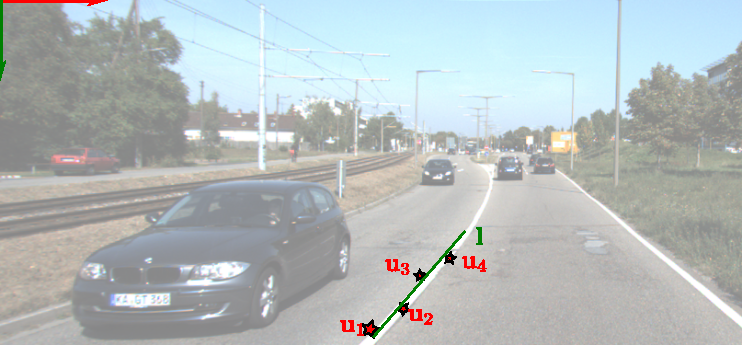
\includegraphics[width=\linewidth]{media/lane-from-points.pdf}
  \begin{align*}
    \ubfx_1 &= [100, 98, 45,1]^\top\\
    \ubfx_2 &= [105, 95, 46, 1]^\top\\
    \ubfx_3 &= [107, 90, 47,1]^\top\\
    \ubfx_4 &= [110, 85, 43,1]^\top
  \end{align*}
  Find  the 3D line such that it is the ``closest line'' passing through
  $\bfx_1, \dots, \bfx_4 \in \bfP^3$.
\end{frame}

\begin{frame}{Parameteric representation through Range space}
  
\end{frame}


\begin{frame}{Homography}
  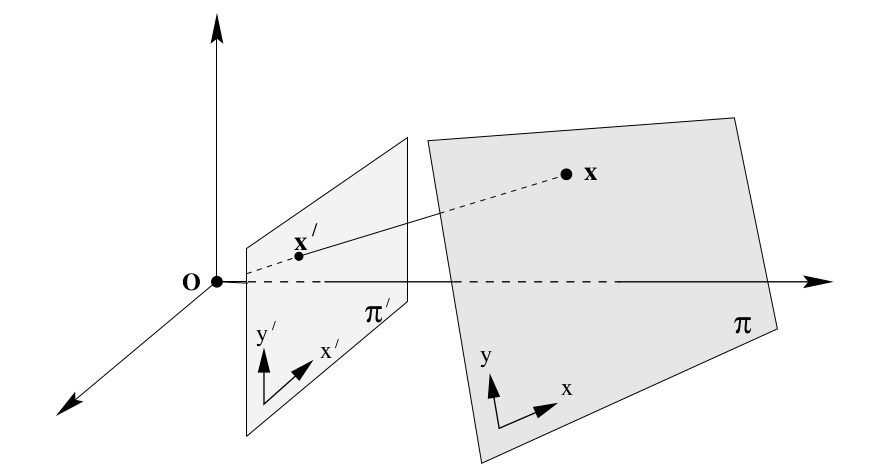
\includegraphics[width=\linewidth]{media/homography-maps-a-line-to-a-line.png}
\end{frame}

\begin{frame}{Examples  of  Homography}
  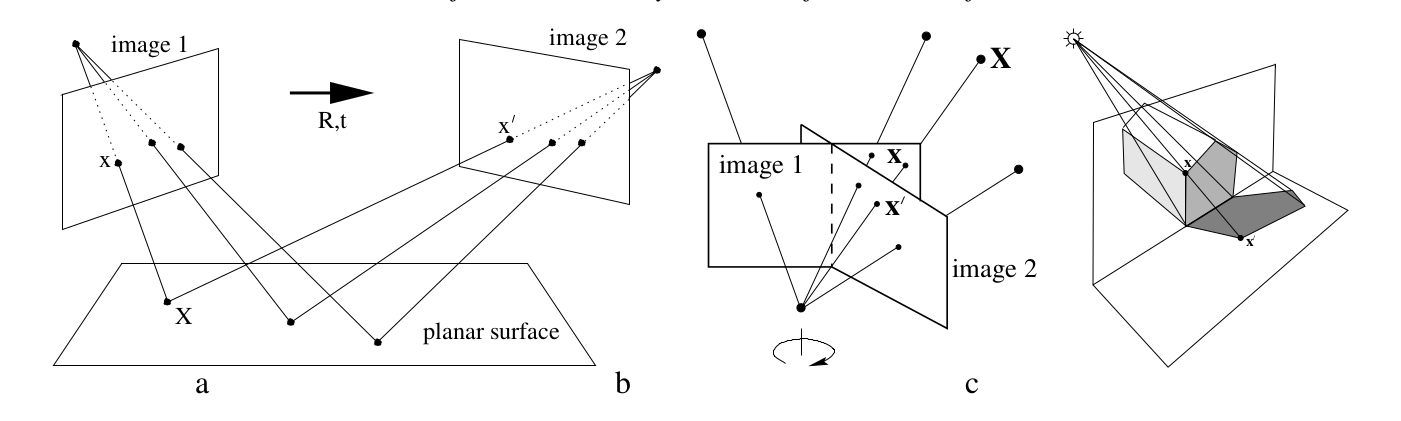
\includegraphics[width=\linewidth]{media/examples-of-homography.png}
\end{frame}

\begin{frame}
  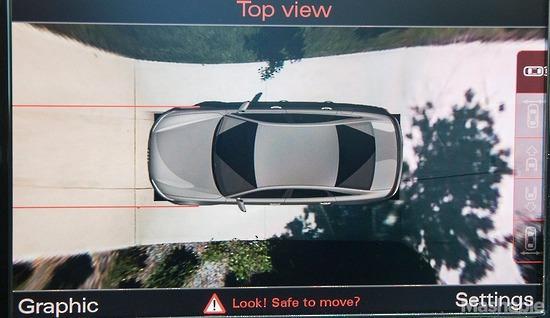
\includegraphics[width=0.60\linewidth]{media/audi top view camera.jpg}
\end{frame}

\begin{frame}{Computing Homography}
  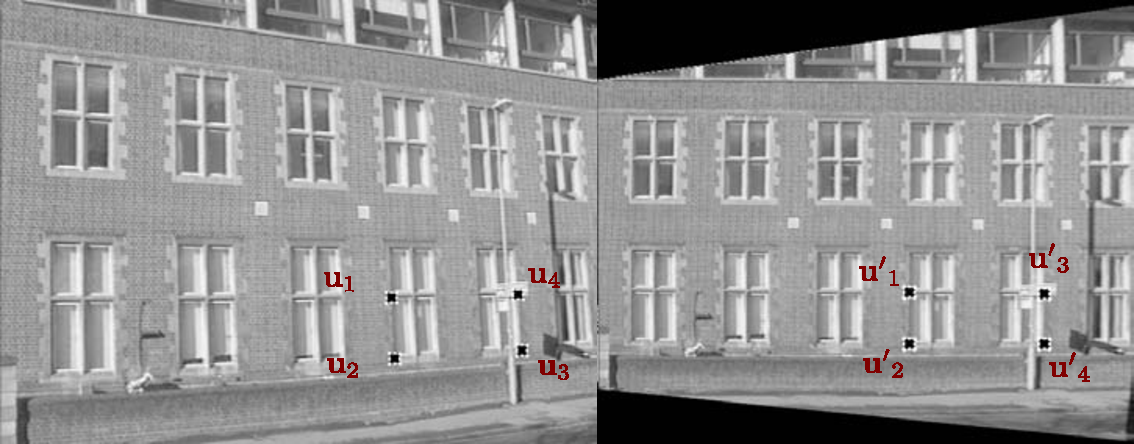
\includegraphics[width=\linewidth]{media/removing-perspective-distortion.png.pdf}
  \begin{align*}
    \ubfu_1 &= [100, 98, 1]^\top&
    \ubfu_2 &= [102, 95, 1]^\top\\
    \ubfu_3 &= [107, 90, 1]^\top&
    \ubfu_4 &= [110, 85, 1]^\top \\
    \ubfu'_1 &= [100, 98, 1]^\top&
    \ubfu'_2 &= [102, 95, 1]^\top\\
    \ubfu'_3 &= [107, 98, 1]^\top&
    \ubfu'_4 &= [110, 85, 1]^\top
  \end{align*}
  Find $H$ such that $\ubfu' = H\ubfu$ for any point on one image to another image.
\end{frame}

\begin{frame}{2D homography}
  Given a set of points $\ubfu_i \in \bbP^2$ and a corresponding set of
  points $\ubfu'_i \in \bbP^2$, compute the projective transformation that takes each
  $\ubfu_i$ to $\ubfu'_i$ . In a practical situation, the points $\ubfu_i$ and   $\ubfu'_i$  are points in two images
  (or the same image), each image being considered as a projective plane  $\bbP^2$.
\end{frame}

\begin{frame}{Solving for Homography }
\end{frame}


\begin{frame}{3D  to  2D camera projection matrix estimation}
  Given a set of points $\bfX_i$ in 3D space, and a set
  of corresponding points $\bfx_i$ in an image, find the 3D to 2D projective
  $\bfP$ mapping
  that maps $\bfX_i$ to $\bfx_i  =  \bfP\bfX_i$.
\end{frame}

\end{document}